 
\chapter{Geometry with GeoGebra}


\section{Introduction to GeoGebra}
\label{sec:geogebra}

GeoGebra is an open source tool that lets you do geometric constructions and also work with algebraic expressions (Hence the Geo and the Gebra in the name).

GeoGebra is available as a an app for your phone, or your computer, or you can just access it via a webpage: \url{https://www.geogebra.org/}.

For doing the labs in this chapter it will be easiest to just use the web interface.  If you want to be able to save your work and/or share your work with others (trust me, this is something you'll want to do) you need to sign in.  You can use an existing sign-on, like Google or Facebook, or you can create a free GeoGebra account.  

Once you are signed in, go to the ``Home'' area and click the ``Start Calculator'' button.

At the top of the page, in the center, there is a selection box that lets you switch between 5 different versions of the GeoGebra calculator.  When you first start the calculator it will be in ``Graphing'' mode.  At the left side of the header area you'll see a ``hamburger'' that lets you access the top-level menu for the app.

\clearpage
\begin{worksheet}{14}{Intro to GeoGebra}{GeoGebra.png}
\begin{enumerate}

\item Start GeoGebra, sign in, and change the mode from ``Graphing'' to ``Geometry''

The interface will now have two large panes.  On the right is the drawing area.  On the left is where you can select from a bunch of different tools.

One source of annoyance is that the system does whatever action is dictated by the tool that is currently active.  So, for example, if you've selected the ``Point'' tool and you then try to move the view, you'll create a point that you hadn't really intended\ldots

One day you'll get used to this, but in the meantime there's an ``undo'' button\ldots

They've recently added a shortcut to get back to the ``Move'' cursor (since that's the most frequent switch we'll want to make, this is very handy)
\vfill

\item When you first enter the ``Geometry'' mode the tool panel will have a very limited number of options.  Expand them by clicking ``More.''  That gives you quite a few more possible tools to use, but at the bottom of the panel you'll find another ``More'' button.  After you click that one, every option will be displayed.  Look through the list of tools and figure out how to draw a regular hexagon.

\vfill

\item Use the ``Point'' tool to draw 5 random points in the drawing area.  

\vfill

\item Locate the shortcut for getting back to the ``Move'' cursor and then practice moving some of your points around.

\vfill

\item Fairly far down in the tool panel, you should find something labelled ``Conic through 5 points.''  Use it to create the conic that passes through your 5 points.

\vfill

\item A conic (a.k.a. a conic section) is the sort of curve that is created where a plane intersects with a cone.  There are four basic types: circles, ellipses, parabolas and hyperbolas.  Hyperbolas are the strangest case because they have two disjoint parts.  Try moving your points around so that you get each sort of conic.

\vfill

\item There are two so-called ``degenerate'' hyperbolas that consist of two lines -- they can either be crossing or parallel.  Move some or all of your points to create both degenerate hyperbolas.

\vfill

\item Right clicking on an object allows you to access a wide range of ``Settings'' for it.  It also gives you the option to ``Show trace'' for the object.  Change your conic's color to something nice.  Also, adjust the thickness of the curve to something you like. To get rid of the ``Settings'' panel, look for the X in the upper-right corner.

\vfill

\item Turn on the ``Show trace'' function for your conic, then play around with moving one or more of the 5 points that were used to define it.  The images you'll generate are pretty cool\ldots

\vfill 

\item Right click again on the conic and open its ``Settings.''  Deselect the radio button that is labelled ``Show Object'' and then close the Settings panel.  Notice that now we're in a pretty bad state.  We've just made the conic invisible, but now there's no way to click on it so we can change its settings (for instance to make it visible again!)  This is one of many places where an alternative view that we haven't yet talked about comes in handy.  Look at the extreme left side of the window.  You should see two icons labelled ``Tools'' and ``Algebra.''  So far we've only looked at the ``Tools'' view.  Clicking it over to ``Algebra'' gives another way of looking at the things we've constructed.  In particular, it should be easy now to make the conic visible again.

\vfill

\item Finally, let's do something with that hamburger in the upper left corner.  Look into those menu options and figure out how to export a graphic file of your construction.  Make graphics of all of the different kinds of conics (including the degenerate cases).

\vfill

\end{enumerate}

\end{worksheet}
\clearpage

\section{Geometric Constructions}

In the classic book ``The Elements'' by Euclid, they layed out the ground rules for doing Geometry.  People have stuck with these basic rules ever since, because figuring out how to construct things with only a limited set of tools is a great intellectual challenge.  The tools are: an unmarked straightedge (not a ruler) and a compass.  When you first open the ``Geometry'' calculator in GeoGebra, only the basic tools are shown -- you can use them to create points, lines and circles.  These basic tools essentially mirror the straightedge and compass from Ancient Greece.  With just these tools you can do quite a lot, for instance, the following diagram illustrates finding the midpoint of a segment.

\centerline{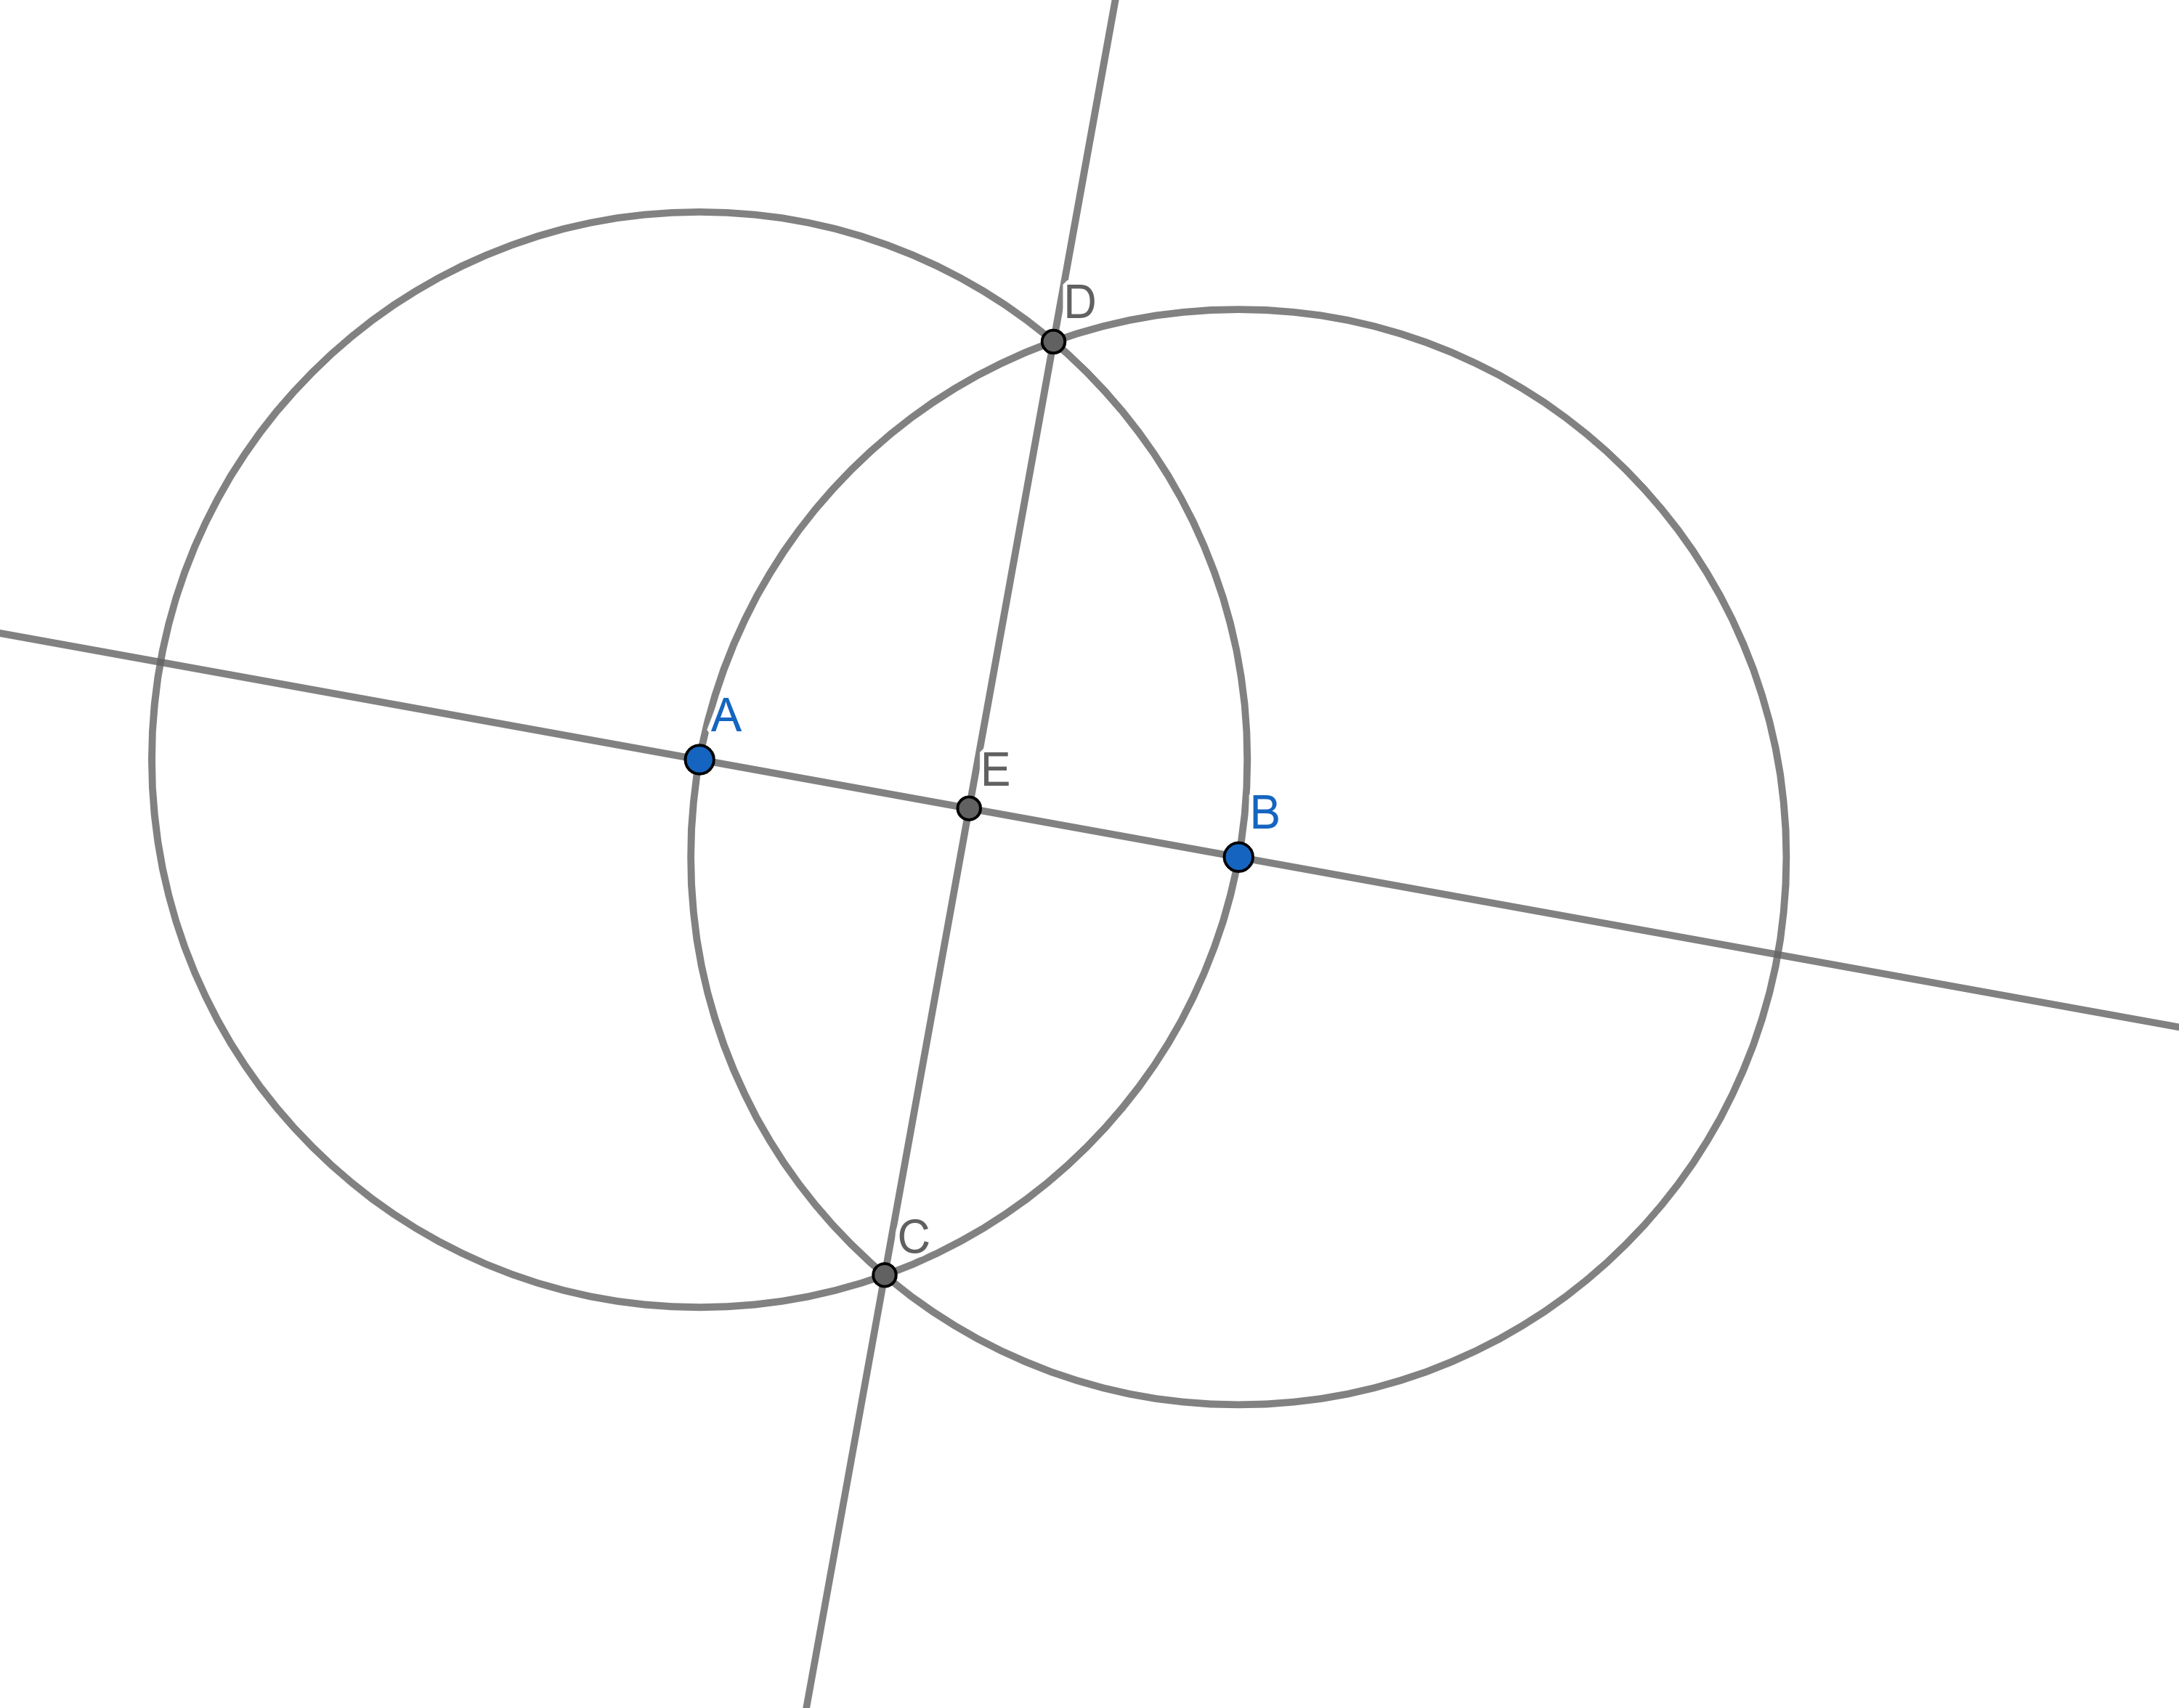
\includegraphics{geogebra-midpoint.png}}

Notice that the construction above also shows how to construct a line that is perpendicular to a given one, and how to construct an equilateral triangle.

When GeoGebra was first released the set of Geometry tools was very limited, but over time they expanded the toolkit -- after all, once you've figured out how to construct a perpendicular bisector, why not just let you click a single button to get one.  Still, some of the tools that are now available stretch the rules of Euclidean geometry.  For instance there is a proof that it's impossible to construct a regular heptagon (that would be a 7-sided polygon with all edge lengths and all angles equal), but there's a tool in GeoGebra that will let you construct a regular polygon with any number of sides that you desire.

In the lab, we're asking you to explore the notion of constructability, but many of the constructions can be accomplished with a single click if you find the right thing to click on.  Please restrict yourself to only using the tools that are ``allowed'' for each exercise.

 \clearpage
 \begin{worksheet}{15}{Geometric Constructions}{GeoGebra.png}
 \begin{enumerate}

\item Start GeoGebra, sign in, and change the mode from ``Graphing'' to ``Geometry''

\vfill

\item When you first enter the ``Geometry'' mode the tool panel will have a very limited number of options.  All but one of the things we'll need for the first task are here -- the additional tool is call ``Intersect'' and you'll need to fully expand the tool panel to find it.  Use points, lines, circles and the ability to construct points at the intersection of two curves to construct an equilateral triangle.

\vfill

\item Create a line and a point that's not on the line.  Can you use the basic tools (constructing lines and circles, finding intersections) to create a line that goes through the point, which is also perpendicular to the original line?

\vfill

\item Once you've completed the previous task, we're justified in letting you use the ``Perpendicular Line'' tool.  Using the basic tools plus ``Intersect'' and ``Perpendicular Line'' construct a square.

\vfill

\item Using the same tools, construct a right triangle where one leg is twice as long as the other.  If we say the short side is one unit long, how long is the hypotenuse of this triangle?

\vfill

\item There is a number you may have heard of called $\phi$ -- the golden proportion.  Its value is $\displaystyle \phi = \frac{1+\sqrt{5}}{2}$.
A golden rectangle is a rectangle whose side are in the golden proportion, so if you can construct a rectangle with sides $2$ and $1+\sqrt{5}$ you will have made a golden rectangle.  Referring to the previous problem, you should be able to do it!

\vfill

\item Let's finish up by exploring some properties of triangles.  Feel free to use any of the tools for these questions.
There are several ways to find a point that can be regarded as the ``center'' of a triangle.  Use Geogebra to construct all of the following:

\begin{enumerate}
	\item The line segments that go from a corner to the midpoint of the edge across from it.  There are three of these, which intersect in a point called the {\em mediant}.
	\item The line segments that are perpendicular to an edge and pass through the point across from the edge.  These intersect in a point called the {\em orthocenter}.
	\item The lines that bisect the angles at each vertex.  These intersect in a point called the {\em incenter}.
\end{enumerate}

\item Create a single triangle and construct the mediant, orthocenter and incenter.  Change the settings so that each type of ``middle'' is constructed with a different color.  Now move the corners around to see if

\begin{enumerate}
	\item it is possible to make all 3 centers coincide.
	\item it is possible to make two centers coincide while the 3rd is different.
\end{enumerate}

\end{enumerate}

 \end{worksheet}
 \clearpage

\section{Parabolas}

You may recall that parabolas are one of the conic sections we played with in lab 14.  As a conic section, a parabola is the intersection of a plane with a cone -- when the plane is parallel to the side of the cone.  There is an alternative way of defining a parabola, which doesn't require us to do anything in 3-d.  Working strictly in the 2-dimensional Euclidean plane we can define a parabola as ``the set of points that are equidistant to a point and a line.''

Let's unpack that definition a little.  There are two ingredients, a line and a point.  The line is called the {\em directrix} and the point is called the {\em focus} of the parabola.  If the focus happens to lie on the directrix we get a degenerate case: the parabola turns into a line.  (This degenerate situation can also be seen in the conic section version of things -- when the plane passes through the tip of the cone.)  To say that a point is equidistant to two things just means that the distance between the point and thing one is the same as the distance between the point and thing two.  Distance between a couple of points is straightforward, but how do we measure the distance between a point and a line?  Short answer: measure perpendicular to the line.

\centerline{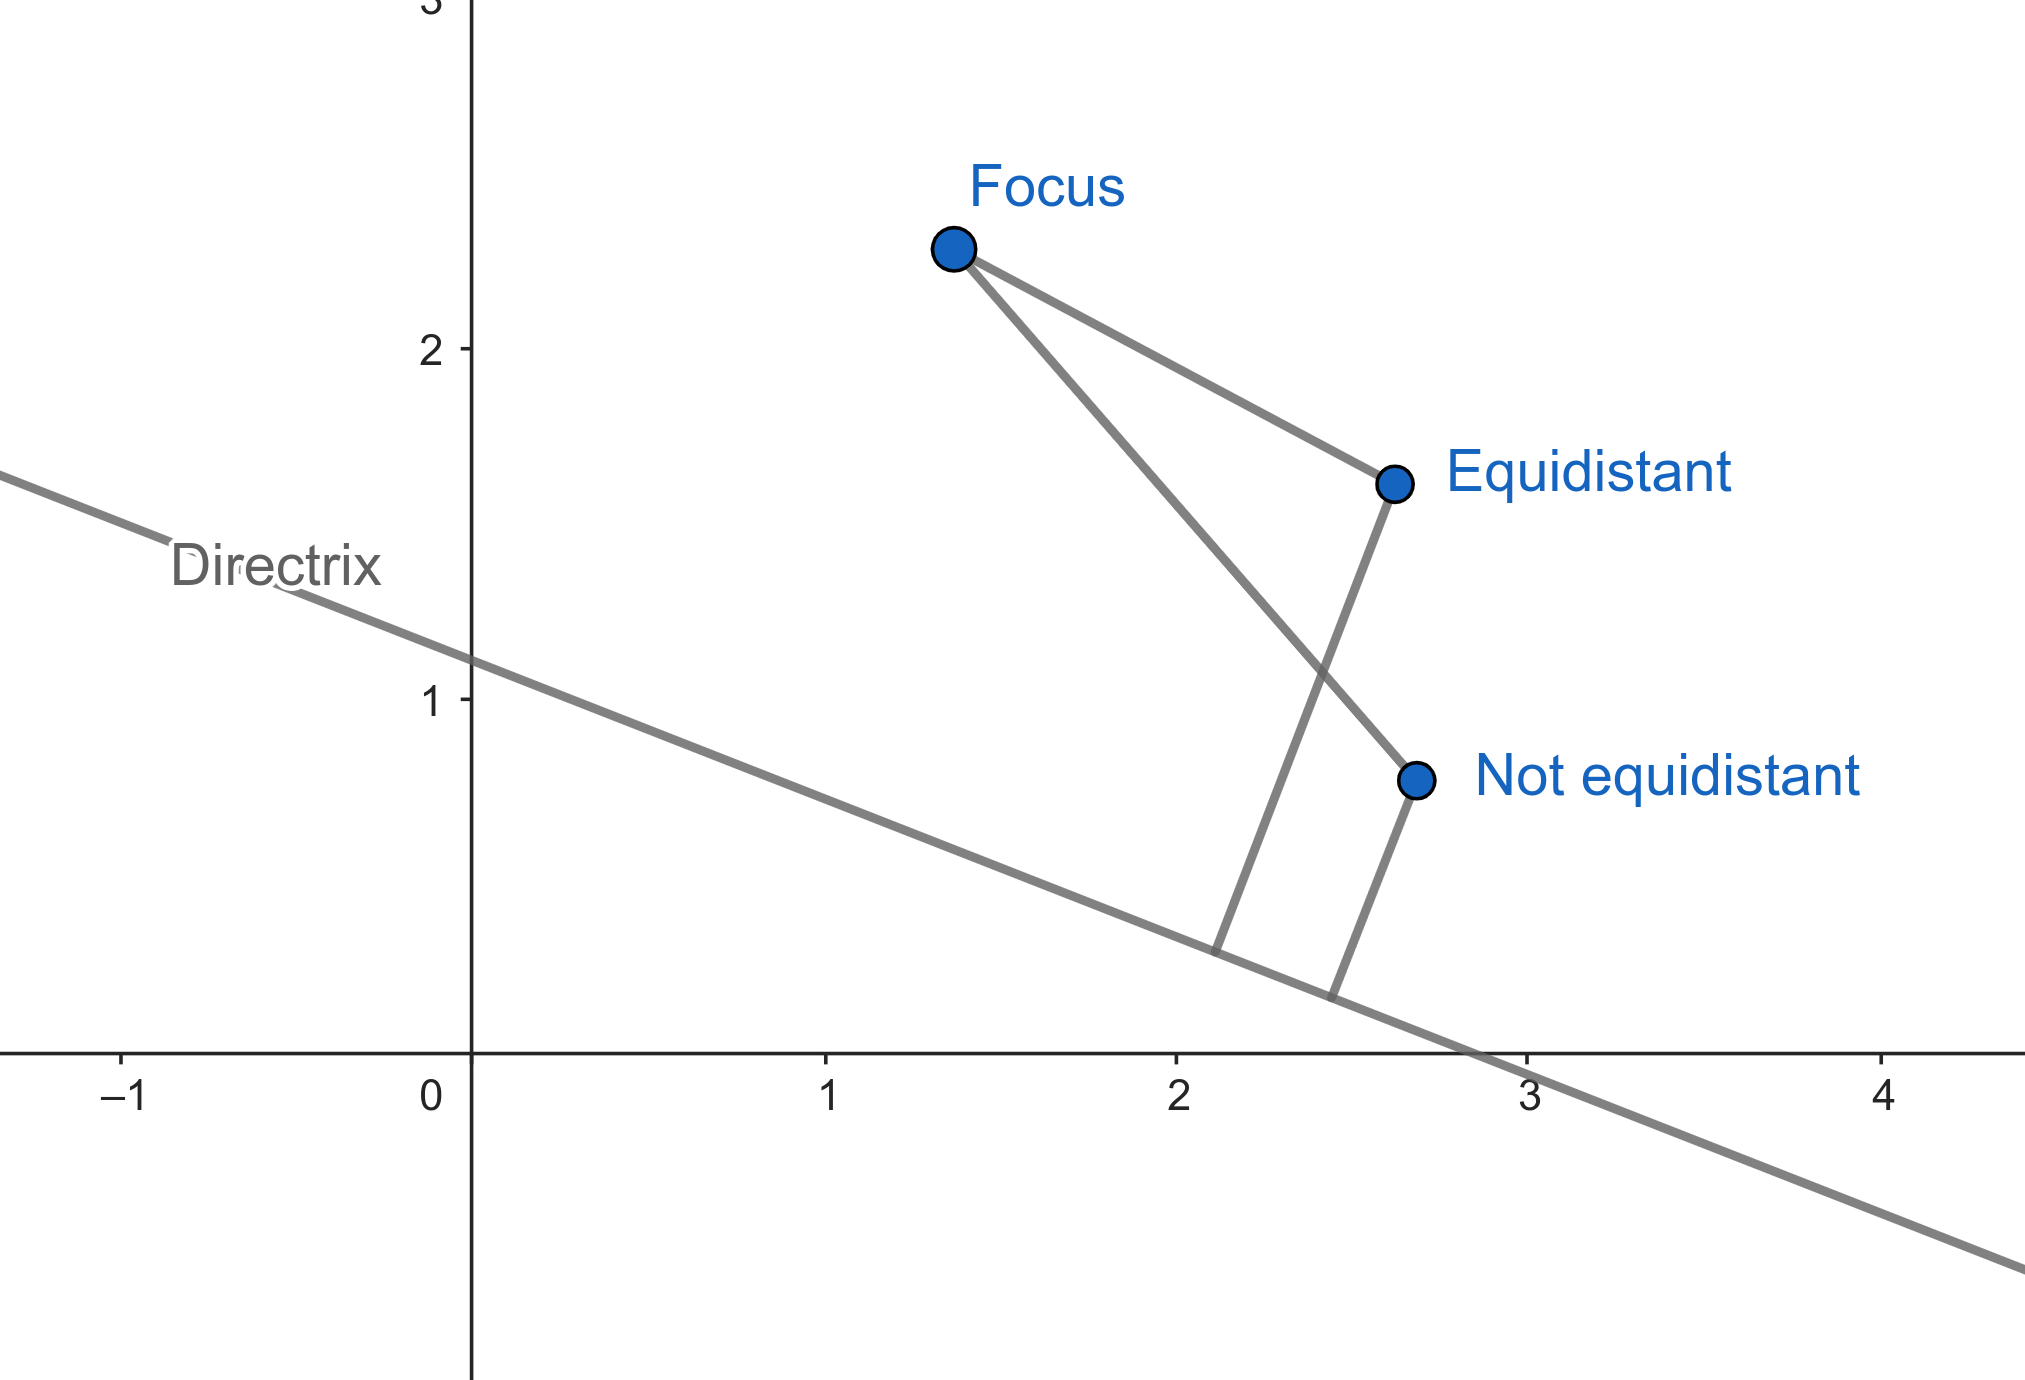
\includegraphics{focus-directrix.png}}

Only one of the points in the figure satisfies the condition of ``being equidistant between the focus and directrix'' so that one would be on the parabola, and the other would not.  Of course, there are many other points which satisfy this ``equidistant'' condition, and when we fill them all in we get our parabola.

\centerline{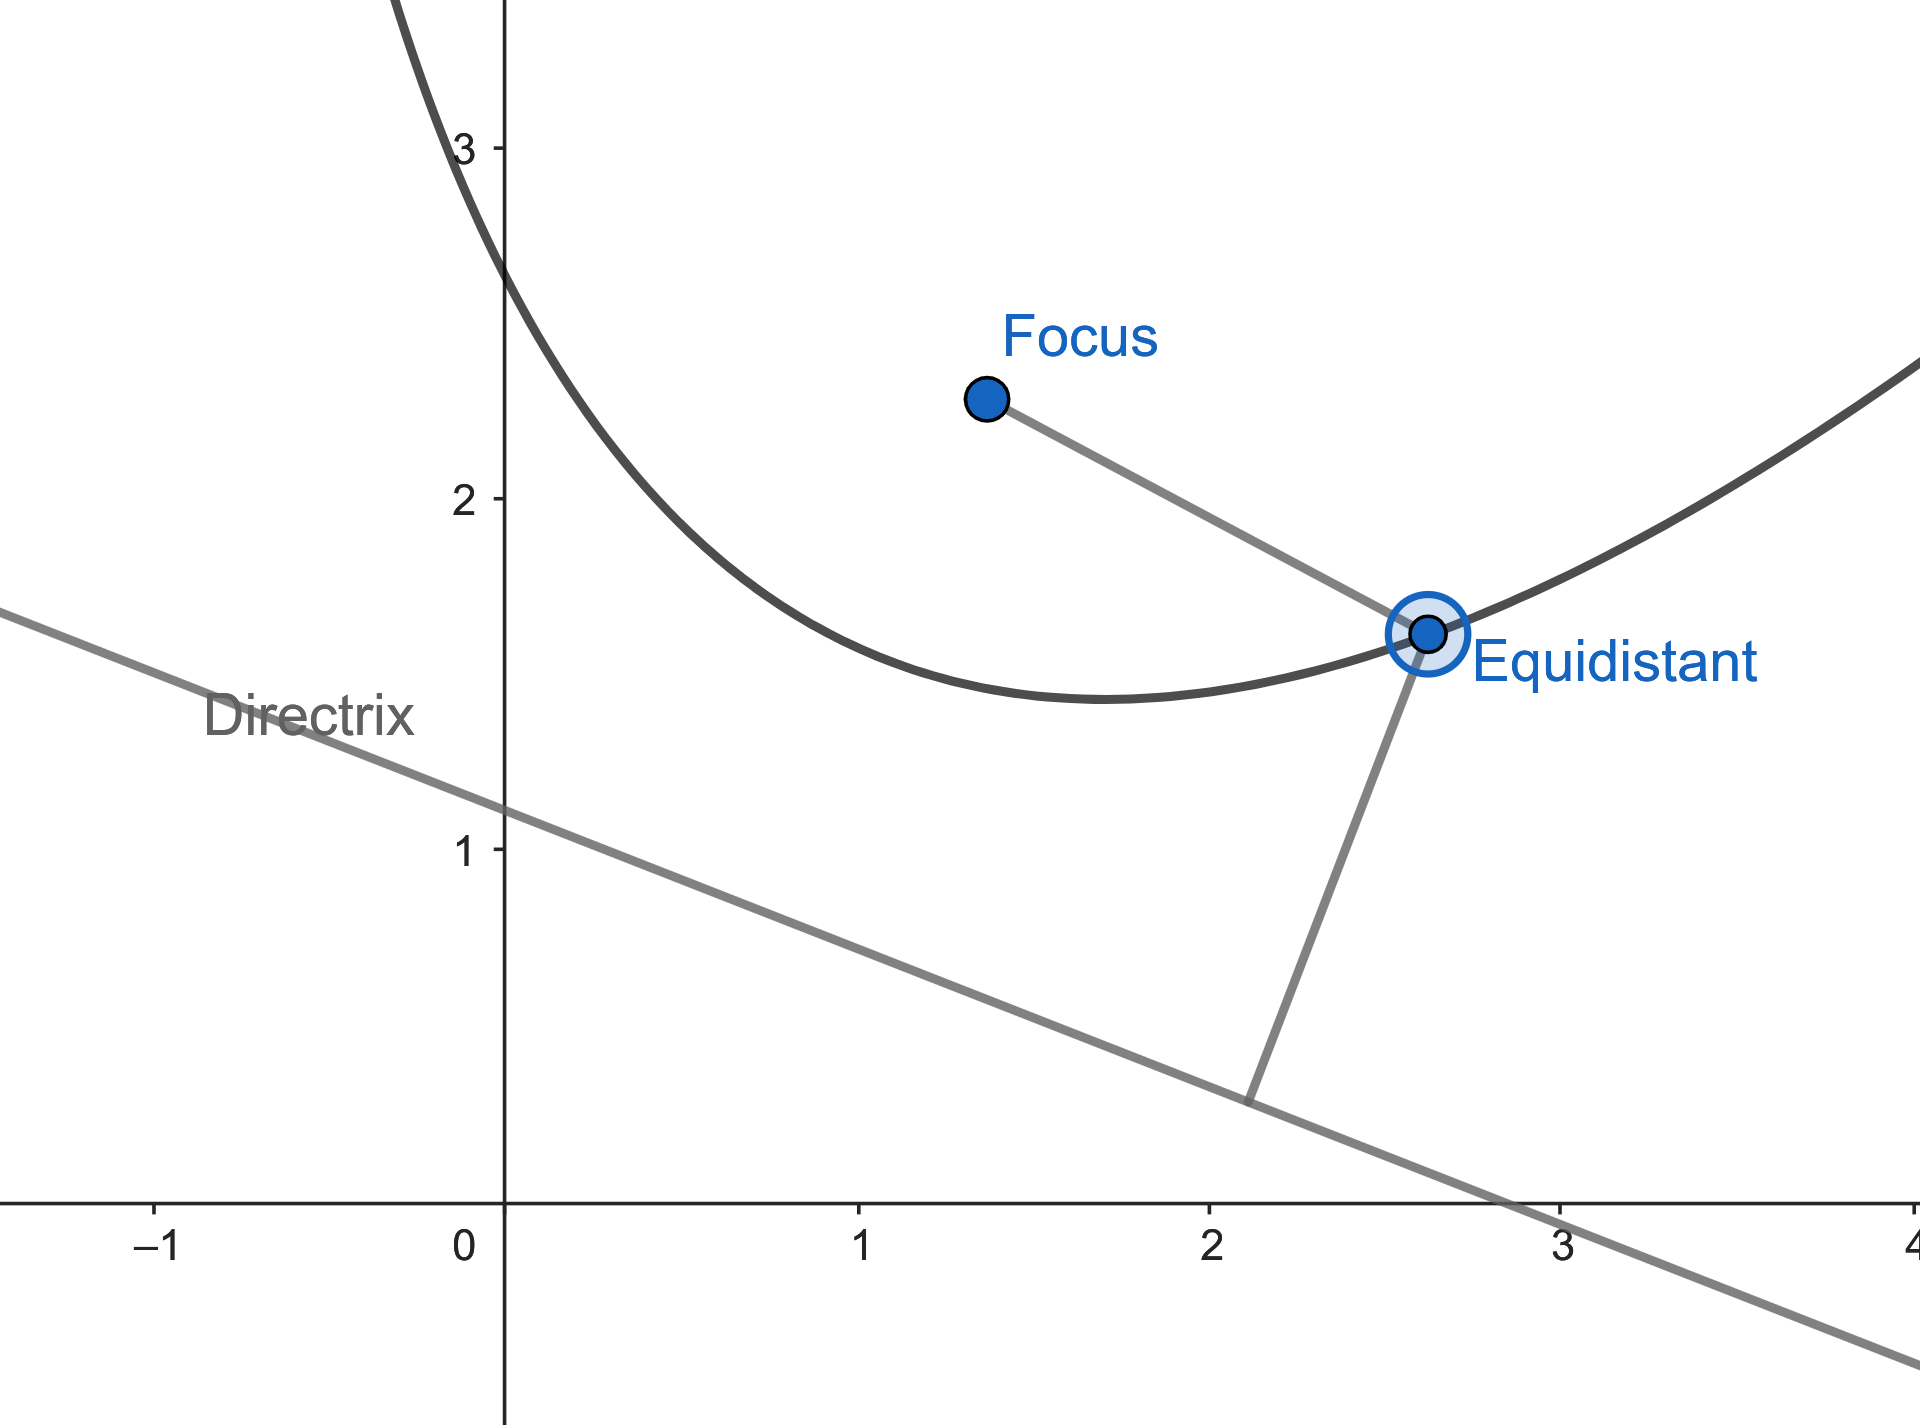
\includegraphics{parabola.png}}

In the lab for this section we'll explore this a bit more.

\clearpage
 \begin{worksheet}{16}{Parabolas}{GeoGebra.png}
 
\noindent In this lab, you will learn how to use GeoGebra to construct a geometric object and how to apply the distance definition of parabola to analyze your construction. Remember, \textbf{a parabola} is the set of points equidistant from a fixed point (the focus) and a fixed line (the directrix). 
\vspace{0.2 in}

In fact, you can create a parabola with nothing more than a sheet of wax (or plain) paper and a single point on the page! The video in this link will show you how one can fold paper to create a parabola: \url{https://www.youtube.com/watch?v=GdJlbNweSVY}. 

\vspace{0.2 in}

But, creasing your paper takes some work. Folding one or two sheets is fun, but what would happen if you wanted to continue testing many different locations for point A? You’d need to keep starting over with fresh paper, folding new sets of creases. Technology can streamline your work. With just one set of creases, you can drag the Focus point to new locations and watch the crease lines adjust themselves instantaneously!


\begin{enumerate}

\item Before trying this on the computer, try doing it with actual paper!

\vfill

\item Start GeoGebra, sign in, and put it in ``Geometry'' mode.

\vfill

\item Use the Line tool to draw a horizontal line near the bottom of the screen. This line AB represents the bottom edge of the paper (the directrix of the parabola).

\vfill

\item Draw a point C above the line, roughly centered between the left and right edges of the screen.	This point will be the focus of your parabola.

\vfill

\item Construct a point D anywhere on the horizontal line and construct the “crease” formed when point D is folded onto point C. There may be other options, but the ``perpendicular bisector tool'' would be a good choice.

\vfill

\item Drag point D along its line. If you constructed your crease line correctly, it should adjust to the new locations of point D.

\vfill

\newpage

\item Select the crease line and choose ``Show trace'' from the right-click menu.

\vfill

\item Drag point D along the horizontal line to create a collection of crease lines.

\vfill

\item To see other cases, you'll want to clear the traces.  Look in the drawing window settings (the gear in the upper right corner of the drawing area) and select ``Clear all Traces.''  Now try moving the focus (point C) to a different location.

\vfill

\item Again, drag point D to create another collection of crease lines.

\vfill 

\item There is a point that actually traces out the parabolas we've been looking at.  It lies at the intersection of the crease line and a line through D, perpendicular to the directrix.  Construct it!

\vfill

\item To create the graph of your parabola, without all the trace lines, check out the ``Locus'' tool.  It draws the path that a point, whose position is determined by something else, will move in.  The tool tip on this is not terribly clear - click the ``Locus'' tool, then the point whose path you want drawn (the locus point) and then the point that controls its motion (point D in this case).

\vfill

\item You can also create the graph of a parabola using the Algebra panel.  Just type \verb+y = x^2+, and you'll get the parabola most people think of when the hear the word ``parabola.''  Challenge: move the directrix and the focus around until you get a close match.

\vfill

\item Final Challenge: What do the think are the actual locations of the focus and the directrix for $y=x^2$?




\end{enumerate}

 \end{worksheet}
\clearpage

\section{More with GeoGebra}

The GeoGebra project started as a tool for doing Geometric constructions.  Over the years, many other capabilities have been added to it.

The selection box at the top/center of the GeoGebra window allows you to choose between several modes: Graphing, 3D Calculator, Geometry, CAS (Computer Algebra System) and Probability.  So far, we've looked mainly at the Geometry mode, but today we'll explore some of the others.

There is a mathematical area that works well as an arena for looking at the Graphing, 3D Calculator and CAS modes.  It's known as ``systems of linear equations.''

The simplest possible ``system'' would have a single equation and there would be only 1 variable too.  For example,

\[ 2x = 8. \]

That's obviously a little too simple!  

Here's a system where there are two variables and two equations:

\begin{align*} x + y &= 14 \\ 
 x - y &= 6 
 \end{align*}
 

That's a little more complicated, but you can probably find the answer by a little bit of ``guess and check.''  We're looking for two numbers that add up to 14 and which differ by 6.

Several years ago when you were first learning about linear equations you would have encountered several ``forms'' for the equation of a line

\begin{itemize}
	\item[slope-intercept form] \rule{0pt}{24pt} \rule{12pt}{0pt} $y = mx + b$
	\item[point slope form] \rule{0pt}{24pt} \rule{12pt}{0pt} $y = m(x - h) + k$
	\item[standard form] \rule{0pt}{24pt} \rule{12pt}{0pt} $ax + by = c$
\end{itemize}

At the time you may have thought that standard form should really be the $y=mx+b$ thing, and that the actual standard form was rather poorly named.  It's at this point (while looking at systems of linear equations) that we see what makes standard form so useful.  One thing that's worth pointing out: in the other two forms, one of the variables is singled out (both of them are solved for $y$), standard form is more egalitarian, neither variable is prefered over the other.

\clearpage
 \begin{worksheet}{17}{More with Geogebra}{GeoGebra.png}
 

\begin{enumerate}

\item Find two numbers that have a sum of 26 and which differ by 8.

\vfill

\item Start GeoGebra, sign in, and put it in ``Graphing'' mode. In the input cells we're going to enter two formulas.  The first is $x+y=26$ and the second is $x-y=8$.
Describe the shapes that are created in words.  What is the significance of the point $(17,9)$ in this picture?

\vfill

\item Consider the pair of linear equations

\[ y = 3x+ 5 \quad \mbox{and} \quad y=-x+3 \]

Graph both of them in the ``Graphing'' window, and find their point of intersection.  What is the significance of this point?

\vfill

\item Here are a couple of linear equations in standard form.

 \[ 3x + 2y = 7 \quad \mbox{and} \quad x - 2y = 5 \]

 Verify that you can get their graphs in GeoGebra without having to first put them in slope-intercept form.  (I.e. GeoGebra is perfectly happy dealing with lines that are in standard form.)  What values of $x$ and $y$ make both of these equations true simultaneously?

 \vfill

\item We've seen that when we graph a linear equation in two variables we get a line in the plane, and when we graph two such things we typically can find a point where they intersect - which is a simultaneous solution to the two equations.  What does this all look like if there are more than two variables?
Switch to the ``3D Calculator'' mode and create a graph of $x+y+z=5$.  Geometrically, what is it?

\vfill

\item Adding a couple of more equations, we get a system of 3 equations in 3 variables:

\begin{align*}
x + y + z &= 5\\
x - y \phantom{ + zz } &= 1\\
x + y - z &= -1
\end{align*}

Create 3D graphs of all three and verify that the point $(1,0,4)$ is the intersection of the 3 planes.

\vfill

\item Sadly, there is no 4D mode for GeoGebra, and to be honest, even in 3D finding a point at the intersection of three planes isn't very easy!  Certainly not as easy as the 2D version of things: finding the intersection of two lines.  This is where the CAS mode comes to the rescue.  We're going to use the CAS mode to work with {\em matrices}.  Matrices are simply tables of numbers -- in the current setting a good way to think of them is as a system of equations with all the decorations removed.  We don't need to write the variables (we always write them in the same order anyway) we just record the coefficients of them.  There's not even a reason to write the $=$ signs - they always come right before the last number in a row (which is whatever is on the right-hand side of the equation).

Here's a very simple system of equations:

\begin{align*}
x + y &= 14\\
x - y &= 6\\
\end{align*}

This is how it looks as a matrix:

\[ \left( \begin{array}{ccc} 1 & 1 & 14 \\ 1 & -1 & 6 \end{array} \right) \]

To enter a matrix into GeoGebra we use nested French braces.

Switch to ``CAS'' mode and enter the following:

\verb+ A = {{1,1,14},{1,-1,6}}+

Press ``Enter'' and it should display a pretty matrix named $A$.

\vfill

\item There is a command in GeoGebra's CAS which is too long to type.  Try typing ``Red'' and then click on the suggestion that pops up.  You want to run a command that looks like

\verb+ReducedRowEchelonForm(A)+

We already know that $x=10$, $y=4$ is the solution to that system.  (If not, take a second to work that out in your head.)  Can you see this solution in the output of that last command?

\vspace{.7in}

\item Final Challenge: Convert the system of linear equations
\begin{align*}
x + y + z &= 5\\
x - y \phantom{ + zz } &= 1\\
x + y - z &= -1
\end{align*}

into a matrix and use \verb+ReducedRowEchelonForm()+ to find its solution.

\vfill

\end{enumerate}

 \end{worksheet}
\clearpage

\section{Projects}

\subsection{A pentagon}

There is a way to create any regular pentagon in GeoGebra.  The challenge of this project is to use the basic Greek geometry tools to construct a regular pentagon -- but do it in GeoGebra.

\subsection{Tilings}

Among the works of the famous Dutch artist M.C. Escher, there are \href{https://mcescher.com/gallery/symmetry/}{many} that illustrate tilings of the plane with recognizable figures.  Such tilings must of necessity involve some of the basic transformations that are found in the GeoGebra toolkit.

\begin{enumerate} 
	\item translations
	\item rotations
	\item reflections
	\item glide-reflections (a combination of translation and reflection)
\end{enumerate}

Use GeoGebra to create an Escher-like tesselation of the plane.  A good intro about how to make a tesselation is \url{https://www.youtube.com/watch?v=Ggk6n-RX4OQ}.

\subsection{Quadric surfaces}

In 2-D we talked about the conic sections.  It turns out that these are also all the types of curves which are the graphs of quadratic relations in two variables.
Use the 3D Calculator in Geobegra to find all of the 3D quadratic surfaces (although, for unknown reasons, in this context, people say ``quadric'' rather than ``quadratic'').
Some judicious Googling might help.
